\documentclass[a4paper,12pt]{report}
\usepackage[utf8]{inputenc}
\usepackage[T1]{fontenc}
\usepackage{graphicx}
\usepackage{enumitem}
\usepackage{geometry}
\usepackage{subcaption}
\geometry{margin=1in}
\makeatletter
\renewcommand{\thesection}{\@arabic\c@section}
\makeatother


\title{\textbf{Installing an OS in a VM}}
\author{Galij Sunuwar}
\date{July 2025}

\begin{document}
% \begin{figure}[h]
%     \includegraphics[]{cover.png}
% \end{figure}
% \newpage
\maketitle

 \tableofcontents
 \newpage

\section {Objective}
\begin{enumerate}
\item To install an OS in a virtual machine manager
\item To document the process of its installation
\end{enumerate}
\section{Introduction}
    \subsection{Virtualization} Virtualization is the process of creating virtual computers on a single physical machine.
    Virtualization is the process of dividing the physical hardware of a computer into many logical parts.
    \newline
    It lets you run several virtual computers on one real computer so that you can use its full power and do multiple tasks at once. 
    Using software such as Hypervisor, virtualization creates an abstraction layer over computer hardware, dividing the components of a single system into multiple virtual machines.
    \newline
    Virtualization is the process of creating a virtual representation of hardware such as server, storage, network, or other physical machines. It supports multiple copies of virtual machines(VMs) to run on one physical machine each with their own operating system and programs.
\subsection{Virtual Machine(VM)}
    After installing virtualization software on your computer, you can set up one or more virtual machines. The Virtual Machines are similar to other applications on our computer. The actual computer is known as 'Host', whereas the virtual computers are known as 'Guests'.
    \newline
    Each guest can have its own operating system. Every guest behaves as a normal computer. It has its own configurations, programs, and settings. The resources, such as the processor, memory, and storage, are all accessed by the virtual machines, but they appear and function exactly like a real computer.
    \newline
    Virtualization is made possible with a hypervisor, also called a virtual machine monitor (VMM). This lightweight software layer manages virtual machines as they run alongside each other.
\newpage
\subsection{Virtualization Software}
Virtualization software allows users to run multiple operating systems or applications on a single physical machine, optimize hardware use, and simplify management.
\newline
These software make it possible for one to achieve virtualization by providing the platform to create virtual machines. One can choose the desired VM specifications, the operating system to be installed, etc.
\newline
Popular options include Oracle VirtualBox, QEMU, VMware Fusion, and Proxmox VE, each offering unique features for different needs.
\newline
\subsubsection{Oracle VirtualBox}
VirtualBox is a general-purpose full virtualization software for x86\_64 hardware (with version 7.1 additionally for macOS/Arm), targeted at laptop, desktop, server and embedded use.
\newline
Some of the main features of Oracle VirtualBox are:

\textbf{Portability}: It is a so-called hosted hypervisor, sometimes referred to as a type 2 hypervisor meaning it requires an existing OS to be installed.
\newline
It can be installed on Linux, Windows or MacOS. It being multi-platform, it is functionally identical on all of the host platforms, and the same file and image formats are used. This enables one to run virtual machines created on one host to be used on another.
\newline
Also, VMs can be easily imported and exported using the Open Virtualization Format which is an industry standard so you can import the OVFs created in a different virtualiztion software too.


\textbf{Guest Addtions: shared folders, seamless windows, 3D virtualizations}: The Oracle VirtualBox Guest Additions are software packages that can be installed inside of supported systems to improve their performance and to provide additional and communication with the host system.
\newline
After the Guest Additions, a virtual machine will support adjustment of video resolutions, seamless windows, accelerated 3D graphics and more. 
\newline
In particular, Guest Additions provide for shared folders, which let you access files on the host system from within a guest machine.


\textbf{Multigeneration branched snapshots}: Oracle VirtualBox can save arbitrary snapshots of the state of the virtual machine. You can go back in time and revert the virtual machine to any such snapshot and start an alternative VM configuration from there, effectively creating a whole snapshot tree.


\textbf{Comprehensive Hardware Support}


\textbf{VM groups}


\textbf{Clean architecture and unprecedented modularity}

\textbf{Remote machine display}
\newpage

\subsubsection{QEMU}
The \textbf{Quick Emulator (QEMU)} is a free and open-source emulator that uses dynamic binary translation to emulate a computer's processor;
 that is, it translates the emulated binary codes to an equivalent 
binary format which is executed by the machine. It provides a variety of hardware and device models for the virtual machine, enabling it to run different guest operating systems.. QEMU can be used with a Kernel-based Virtual Machine (KVM) to emulate hardware at near-native speeds. Additionally, it supports user-level processes, allowing applications compiled for one processor architecture to run on another.
\newline
QEMU supports the emulation of x86, ARM, PowerPC, RISC-V, and other architectures.
\newline
QEMU is free software developed by Fabrice Bellard. Different componenets of QEMU are licensed under the GNU General Public License (GPL), BSD license, GNU Lesser General Public License (LGPL), or other GPL-compatible licenses.
\newline
It has mutliple operating modes:

\begin{itemize}
    \item User-mode Emulation
    \item System Emulation
    \item Hypervisor Support

\end{itemize}
Supported disk image formats:\
\begin{itemize}
    \item Linux cloop
    \item Bochs
    \item macOS Universal Disk Image Format (.dmg)
    \item VirtualBox Virtual Disk Image (.vdi)
    \item Virtual PC Virtual Hard Disk (.vhd)
    \item Virtual VFAT
    \item VMware Virtual Mahcine Diks (.vmdk)
    \item Raw images (.img)
    \item CD/DVD images (.iso)
    
\end{itemize}
It has the following features:

\begin{itemize}
    \item Full System Emulation
    \item User-Mode Emulation
    \item Hardware Virtualization
    \item Snapshotting
    \item Live Migration
    \item Versatile Disk Image Formats
\end{itemize}
\subsection{Use Cases}
    \begin{enumerate}
        \item OS Testing
        \item Software Development and Testing
        \item Server and Network Manipulation
        \item Safe environment for malware analysis
    \end{enumerate}


\section{Tools/ Requirements}
\textbf{Manjaro} is a free and open-source linux distribution based on the Arch Linux operating system with a focus on user-friendliness, accessibility, and imporoved software testing and stability compared to its upstream sources. It uses a rolling release update model with Pacman-derived package managers. 
\newline
I chose this distribution as it was easy to set up and use and it was suitable for both beginners and experienced users. It was also pretty easy to install.
\newline
I used \textbf{Oracle’s Virtualbox} as the virtualization software to create a virtual machine for installing manjaro. The flavour of manjaro I chose was the \textbf{XFCE} version which is known to be lightweight compared to its other versions.
\section{Procedure}
\subsection{Installing Virtualbox}
There are various programs that offer virtualization and Orcale's Virtualbox Manager has a beginner-friendly UI so I decided on Virtualbox.
\begin{figure}[h]
    \centering
    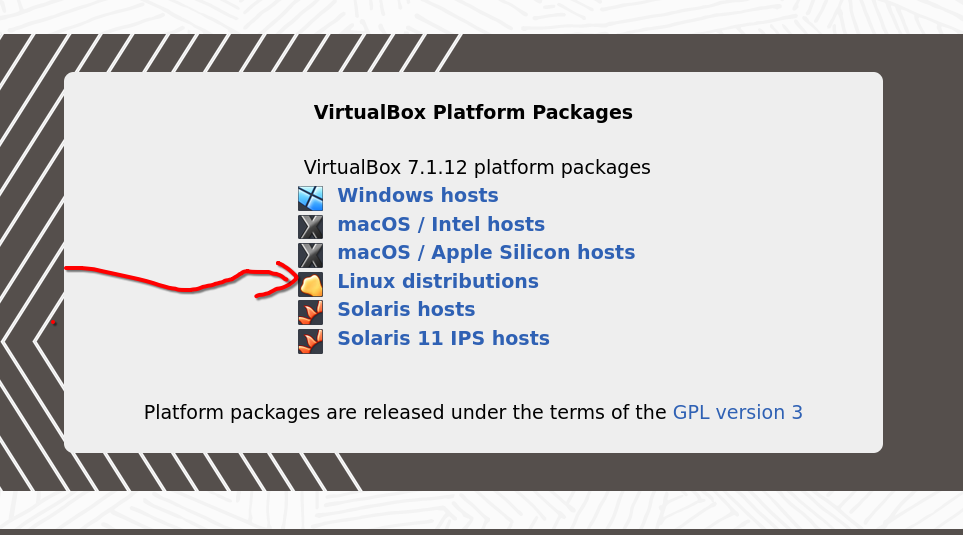
\includegraphics[height=250px]{virtualbox.png}
    \caption{Oracle VirtualBox Webpage}
\end{figure}
\subsection{Selecting the OS}
I decided to install Manjaro OS based on Arch Linux, which uses the Pacman package manager, running XFCE as the desktop environment as it is lightweight to its KDE counterpart.

\begin{figure}[h]
    \centering
    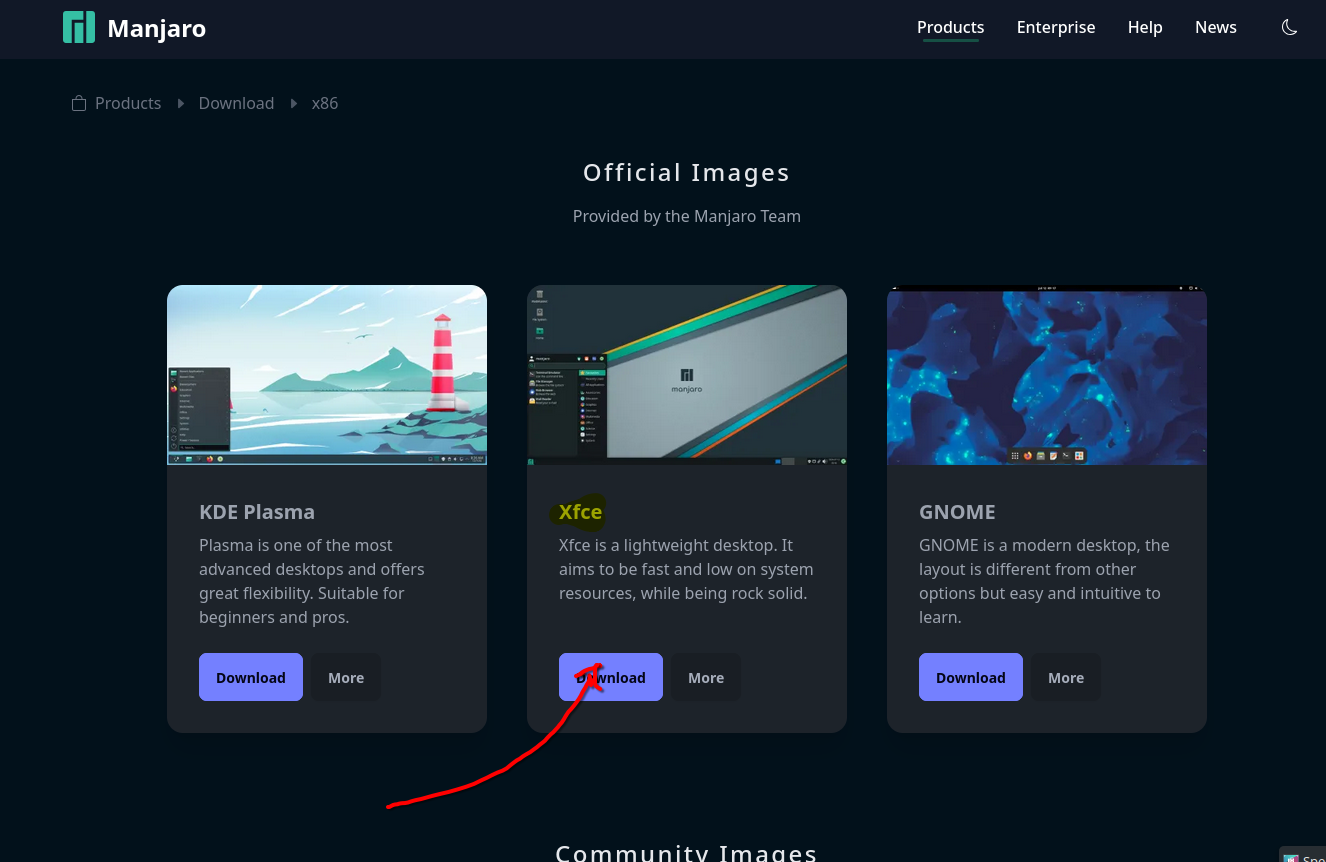
\includegraphics[height=250px]{./manjaro.png}
    \caption{Official Manjaro Webpage }
\end{figure}
\newpage
\subsection{Creating the VM}
Oracle VirtualBox provides a beginner-friendly interface along with complex features to run OS on.
\newline
\begin{figure}[h]
    \centering
    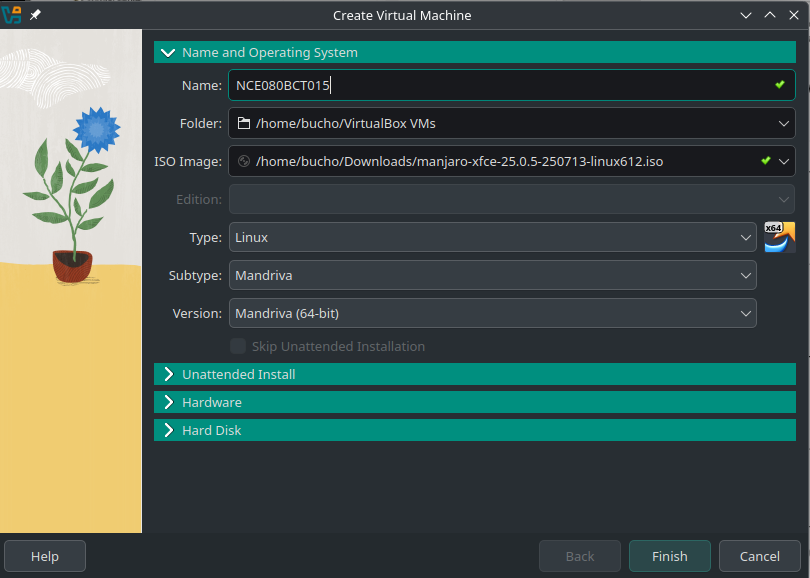
\includegraphics[width=1\linewidth]{creation.png}
    \caption{Naming the VM}
    \label{fig3}
\end{figure}
\newline
I began by naming my VM as well as setting the ISO image I downloaded as shown in Figure 3.
\newline
Then, came the step of allocating the required memory, processors as well as the storage to the VM. 
Note: No more than the host's specifications could be provided to the guest.
\newpage
\begin{figure}[h]
    \centering
    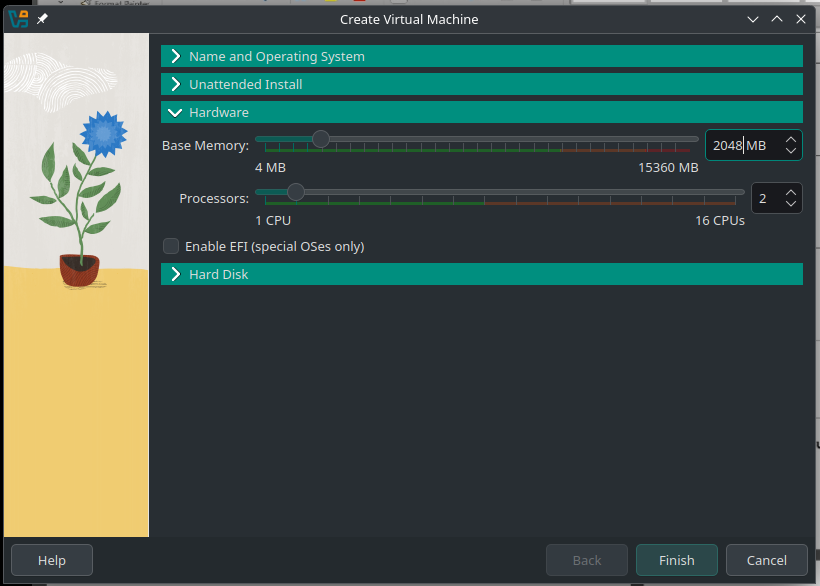
\includegraphics[width=0.7\linewidth]{sys_config.png}
    \caption{Memory and Processor allocation}
    \label{fig4}
\end{figure}
\begin{figure}[h]
    \centering
    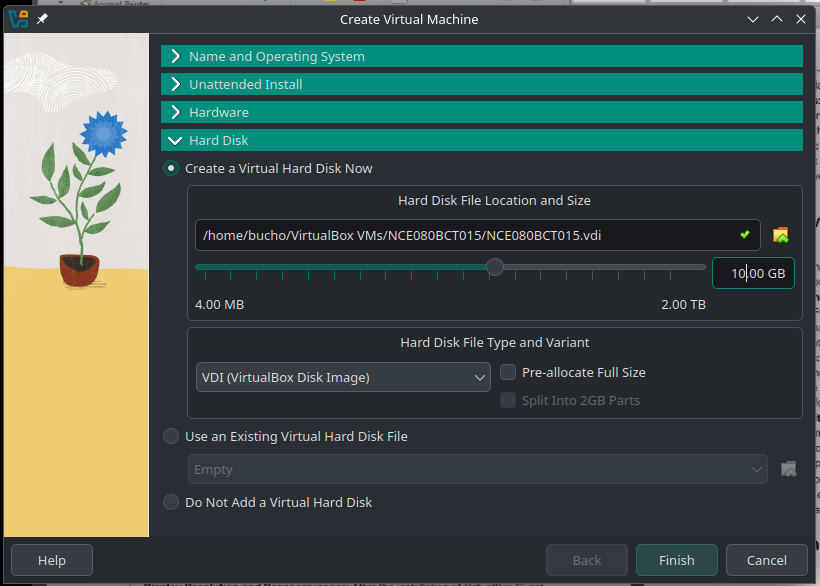
\includegraphics[width=0.7\linewidth]{storage_allocation.png}
    \caption{Storage allocation}
    \label{fig5}
\end{figure}
\newpage
And finally, I setup the video memory and configured the network of the VM. 
\begin{figure}[h]
    \centering
    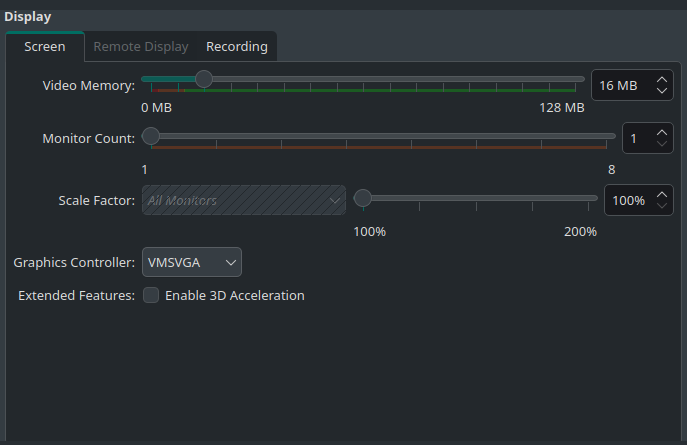
\includegraphics[width=0.7\linewidth]{video_mem.png}
    \caption{Video Memory Allocation}
    \label{fig6}
\end{figure}
\begin{figure}[h]
    \centering
    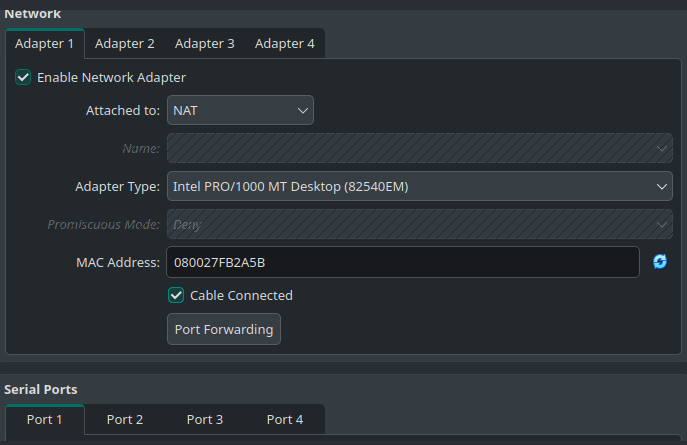
\includegraphics[width=0.7\linewidth]{network_config.png}
    \caption{Network configuration}
    \label{fig7}
\end{figure}
\newpage
After completely setting up the VM, I was ready to boot it and install Manjaro on it.
\begin{figure}[h]
    \centering
    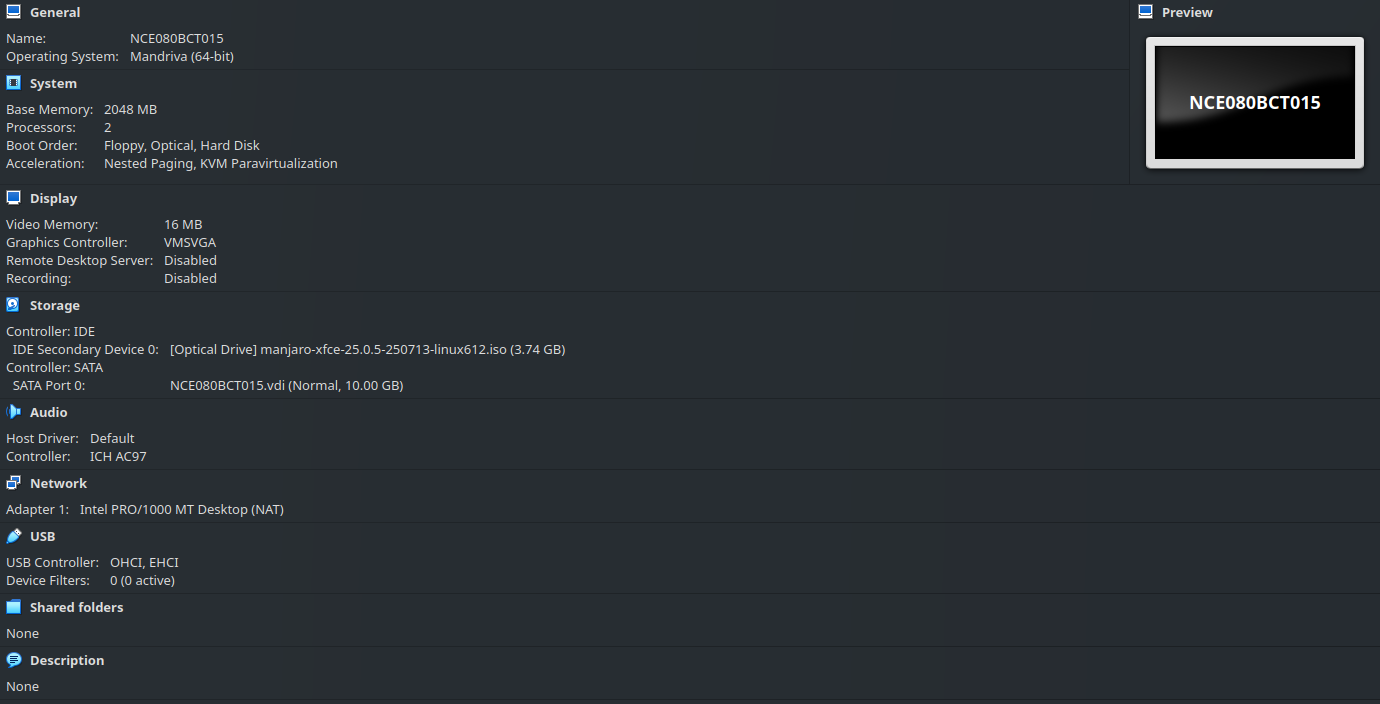
\includegraphics[width=1\linewidth]{sys_summary.png}
    \caption{System Summary}
    \label{fig8}
\end{figure}
\newpage

\subsection{Booting the VM}
\begin{figure}[h]
    \centering
    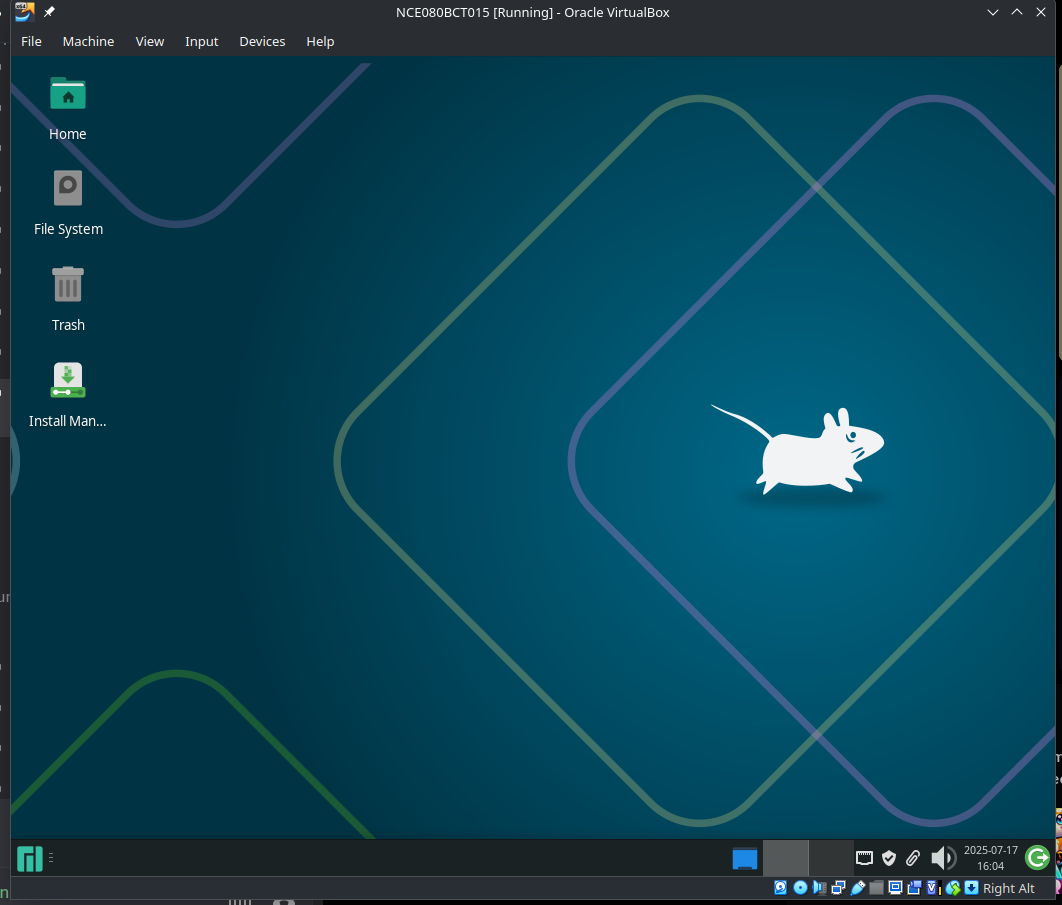
\includegraphics[width=0.5\linewidth]{vm_boot.png}
    \caption{VM Boot}
    \label{fig9}
\end{figure}

\subsection{Installing the OS}
Since, most of the linux distributions provide a Live CD/DVD, one can boot into the OS and try how it functions before actually it into the system.
\newline
The OS was installed in the same way one would install Manjaro on a normal computer.
\newline
\begin{figure}[h]
    \centering 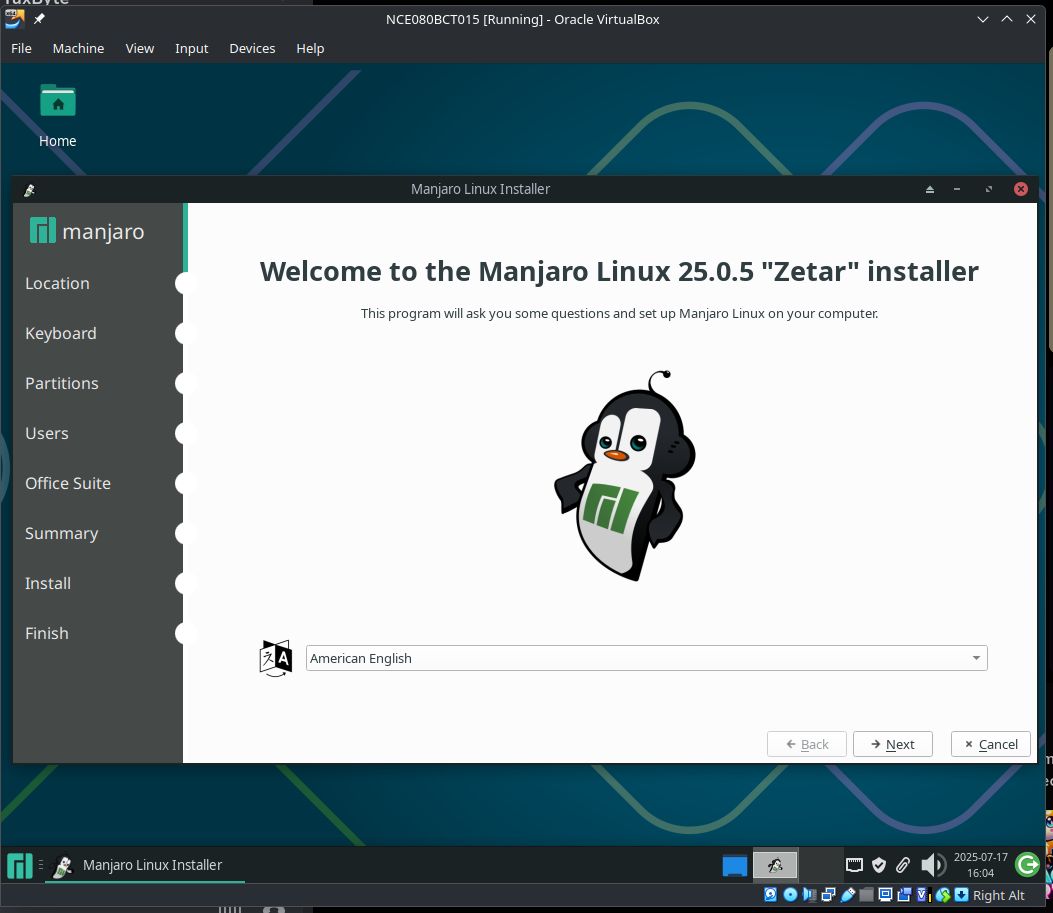
\includegraphics[width=0.6\linewidth]{install1.png}
    \caption{Choosing the Language}
    \label{fig10}
\end{figure}


American English was chosen as the default language to be used for the system. 

\begin{figure}[h]
    \centering
    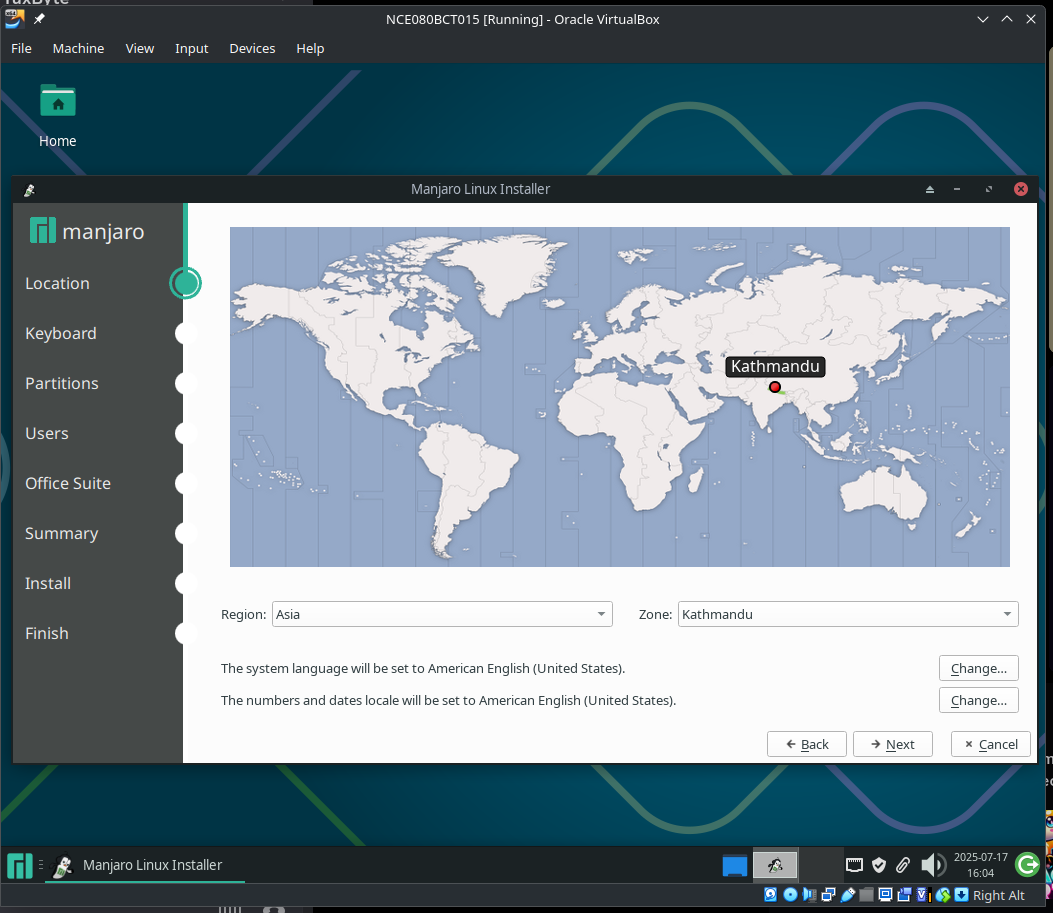
\includegraphics[width=1\linewidth]{install2.png}
    \caption{Selecting the region}
    \label{fig11}
\end{figure}
\newpage
The local region was set according to the connected network while the system language and the dates locale was set to American English.
\newpage
\begin{figure}[h]
    \centering
    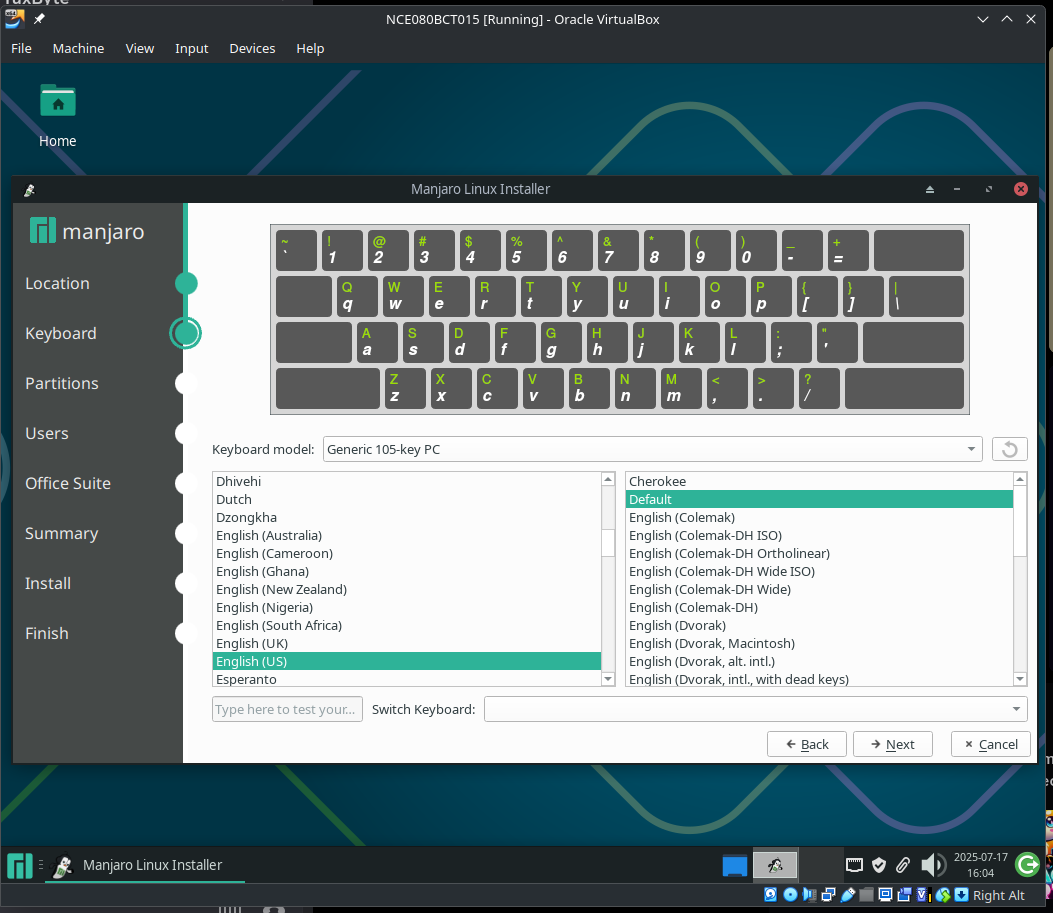
\includegraphics[width=1\linewidth]{install3.png}
    \caption{Choosing the keyboard layout}
    \label{fig12}
\end{figure}

The QWERTY layout in the English(US) format was chosen for the keyboard as it mirrored the original setup.
\newpage
\begin{figure}[h]
    \centering
    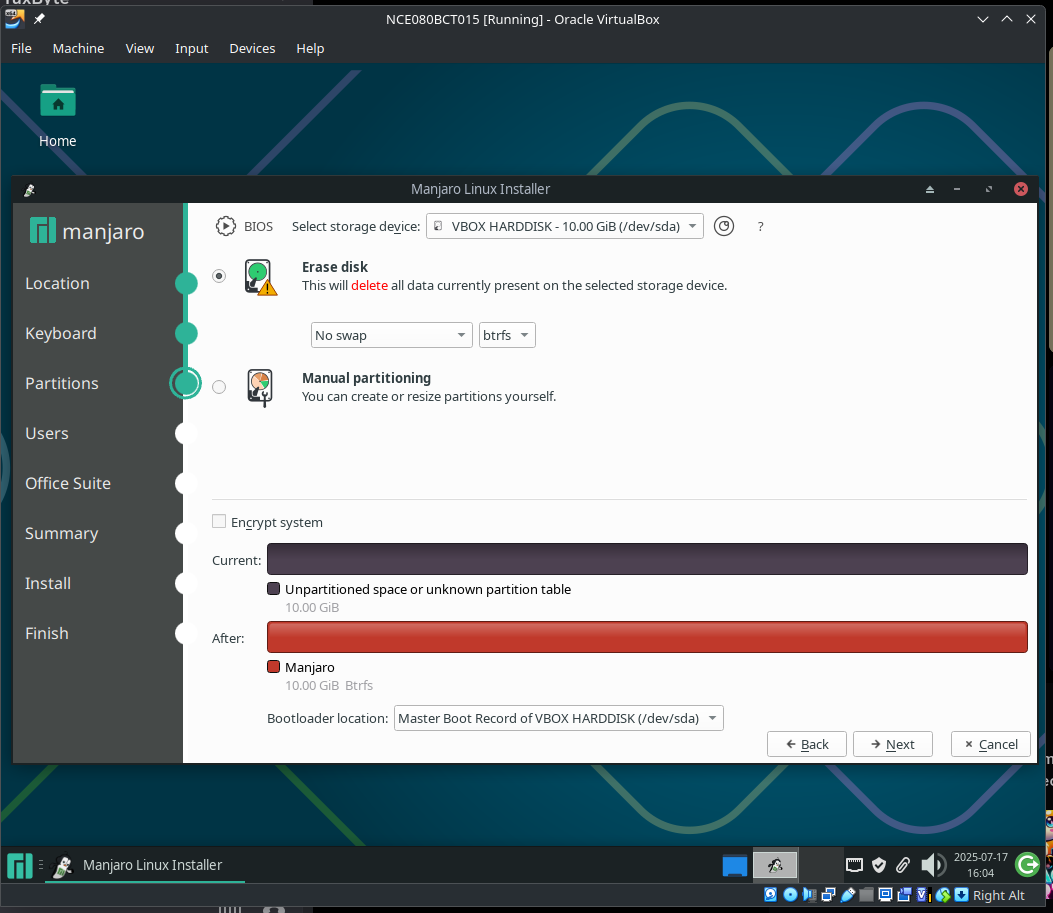
\includegraphics[width=1\linewidth]{partition.png}
    \caption{Partitioning the system}
    \label{fig13}
\end{figure}
The disk was completely erased and wholly used for installing Manjaro OS but partitioning for keeping the root, home and boot partitions separate could be done manually.
\newpage
\begin{figure}[h]
    \centering
    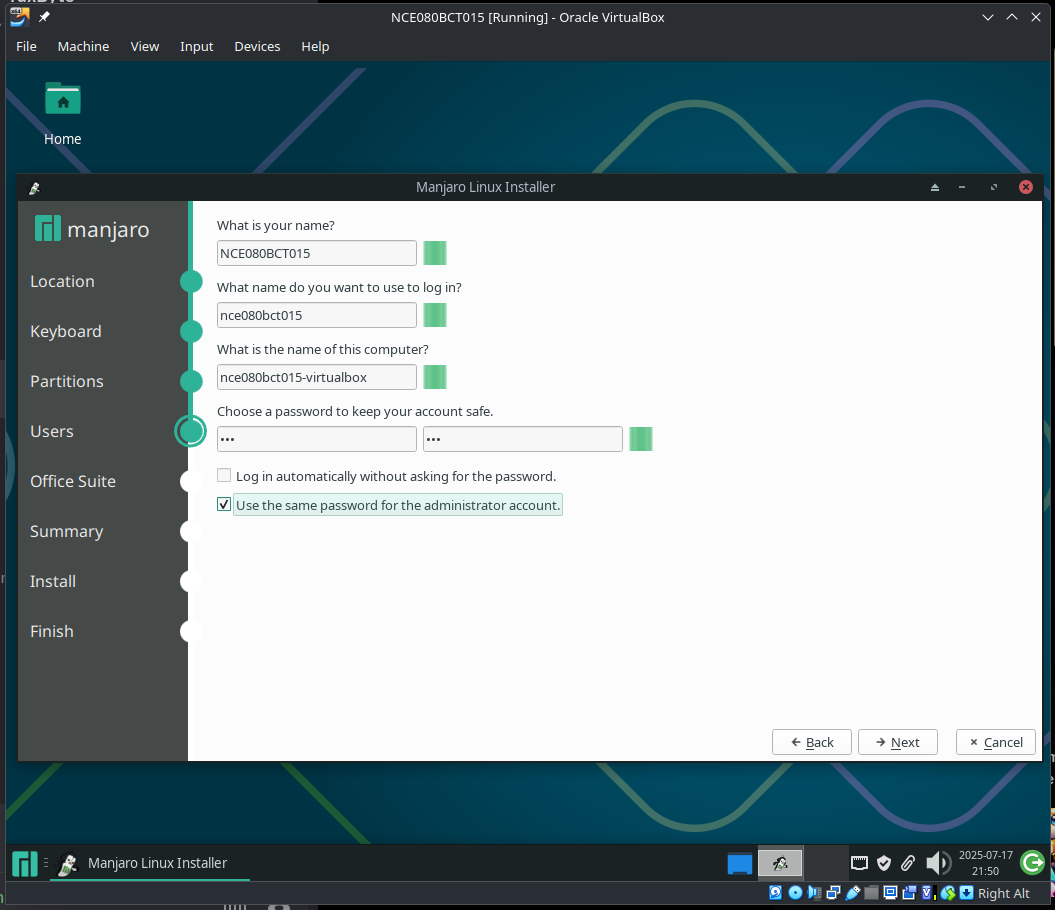
\includegraphics[width=1\linewidth]{user_config.png}
    \caption{Configuring the User}
    \label{fig14}
\end{figure}
A user for Manjaro after installation was configured by setting the name and the password. Additionally, the same password for the user was set as the password for the admin or the root account.
\newpage

\begin{figure}[h]
    \centering
    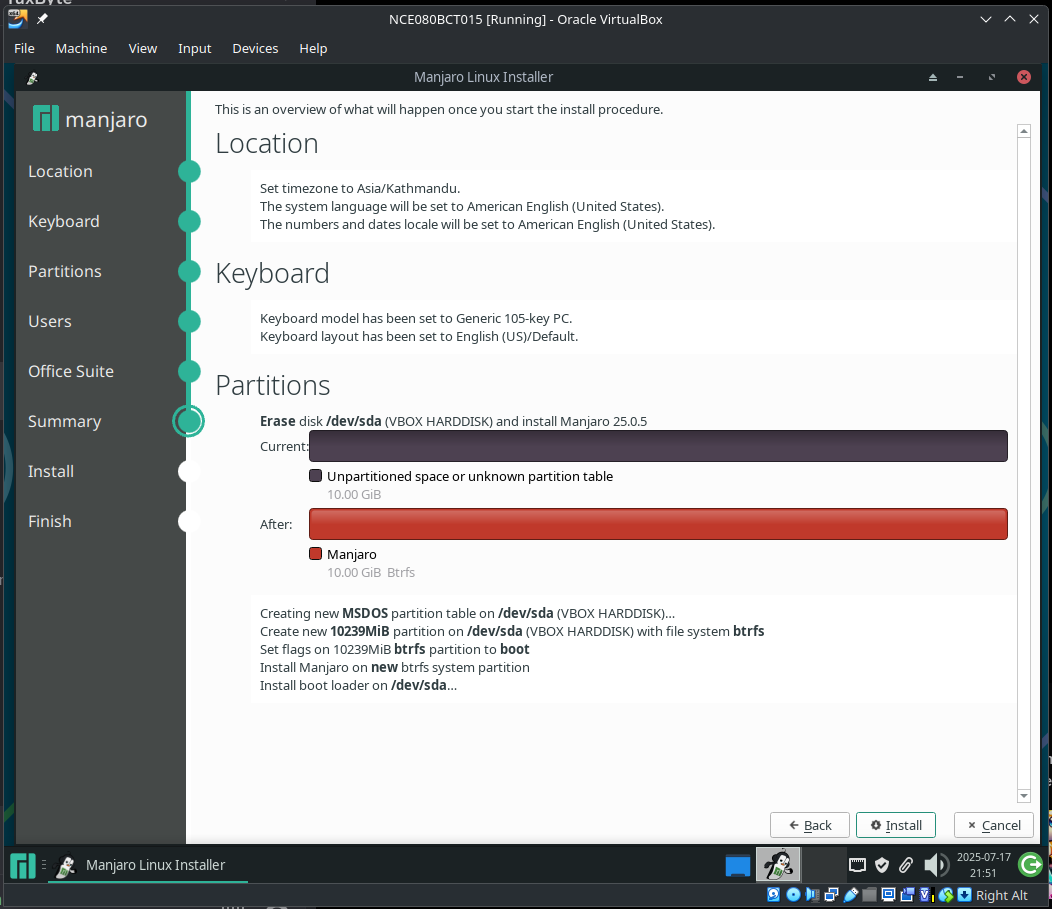
\includegraphics[width=1\linewidth]{install_summary.png}
    \caption{Summary of the system}
    \label{fig15}
\end{figure}
The summary of the installation to be done as well as the things we set up was displayed on a summary page before we moved on to the installation.
\newpage
\begin{figure}[h]
    \centering
    \begin{subfigure}[b]{0.3\textwidth}
        \centering
        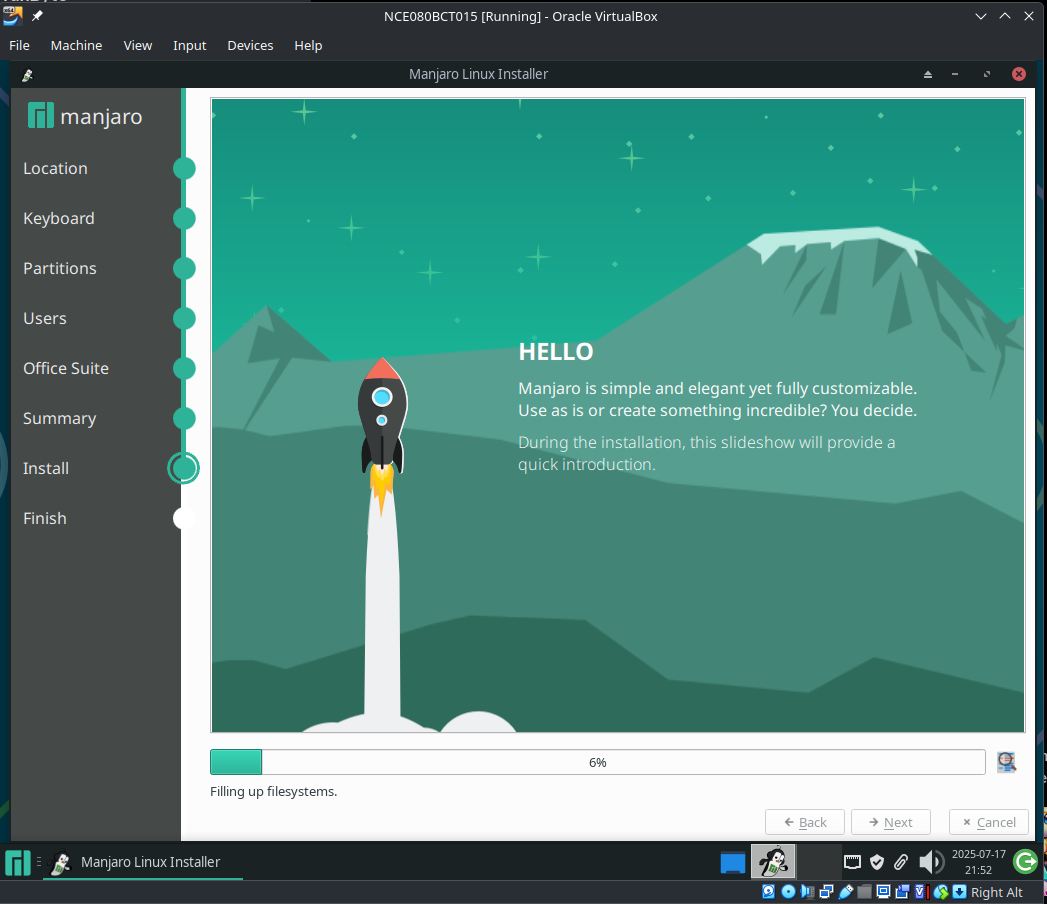
\includegraphics[width=\linewidth]{installation.png}
        \caption{Installation 1}
        \label{fig16}
    \end{subfigure}
    \hfill
    \begin{subfigure}[b]{0.3\textwidth}
        \centering
        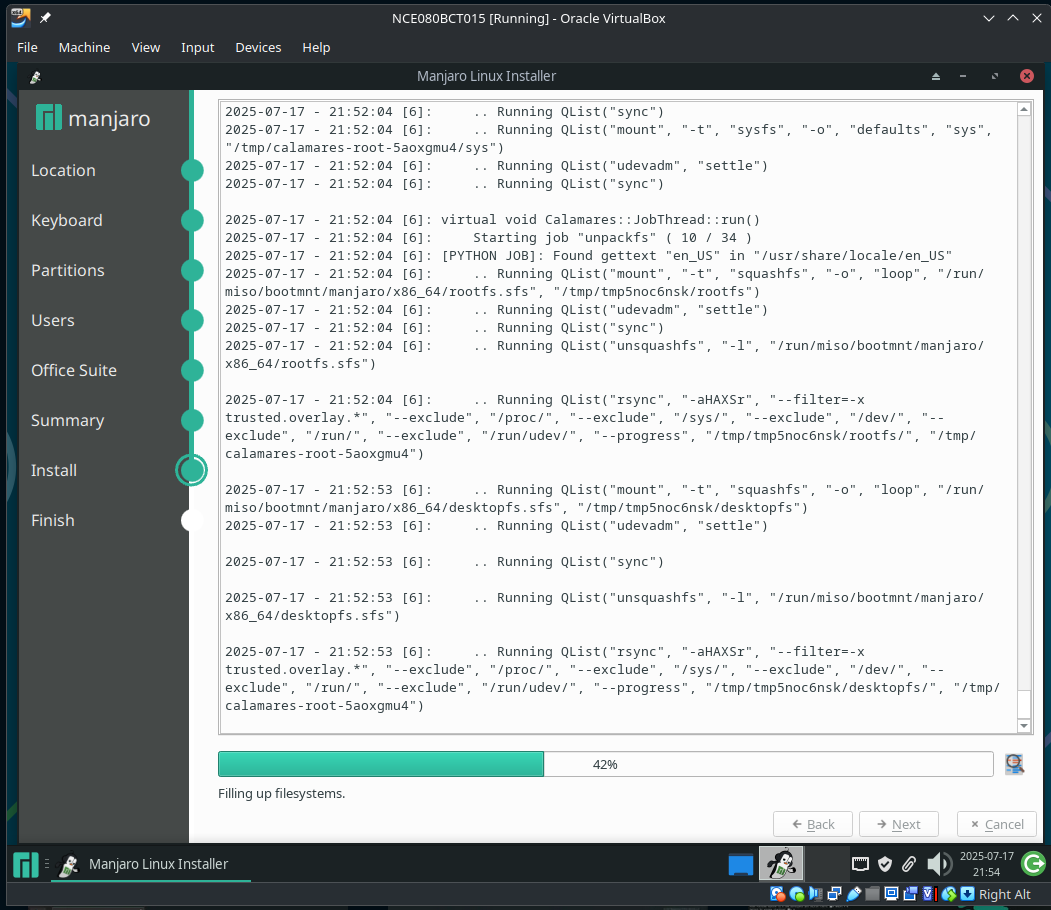
\includegraphics[width=\linewidth]{installation2.png}
        \caption{Installation 2}
        \label{fig17}
    \end{subfigure}
    \hfill
    \begin{subfigure}[b]{0.3\textwidth}
        \centering
        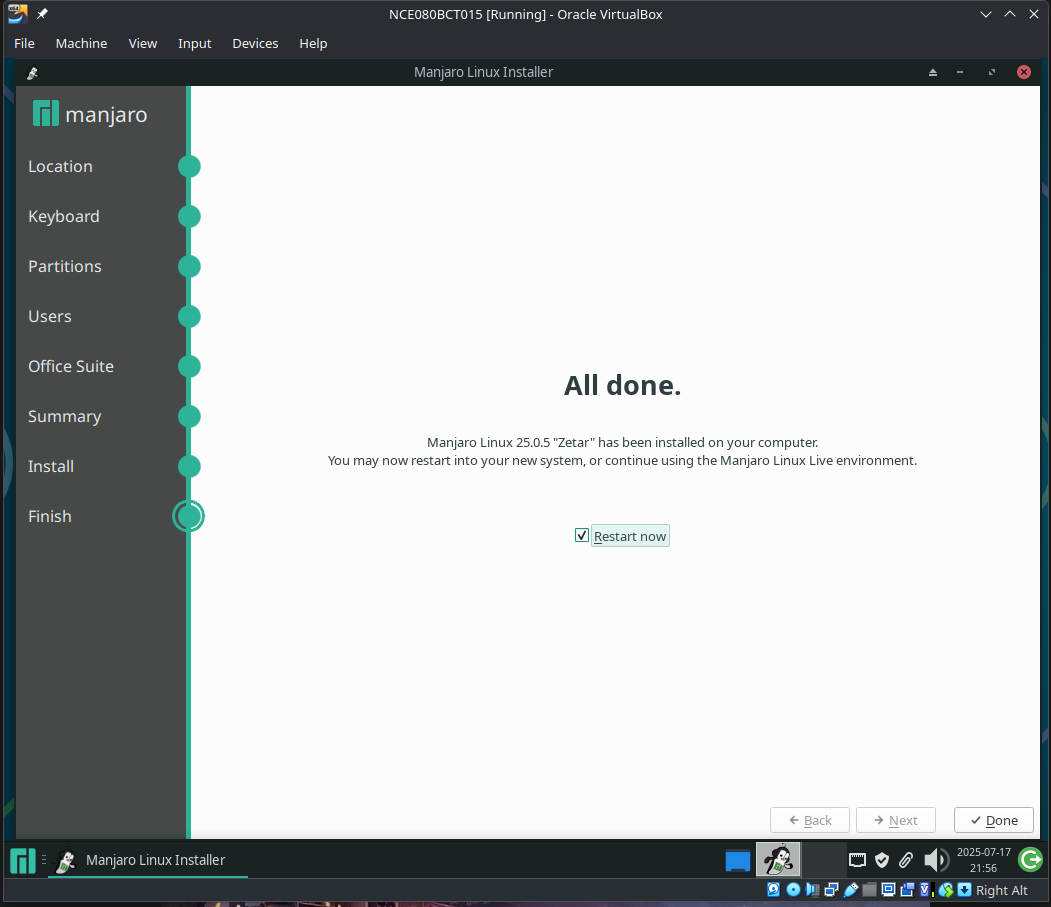
\includegraphics[width=\linewidth]{installation_finish.png}
        \caption{Installation Finish}
        \label{fig18}
    \end{subfigure}
    \caption{Steps of the installation process}
\end{figure}
After proceeding from the installation summary, the installer started installing the OS according to the settings we configured and after completion we rebooted the VM for post install configuration. 
\subsection{Post-Install Configuration}
\begin{figure}[h]
    \centering
    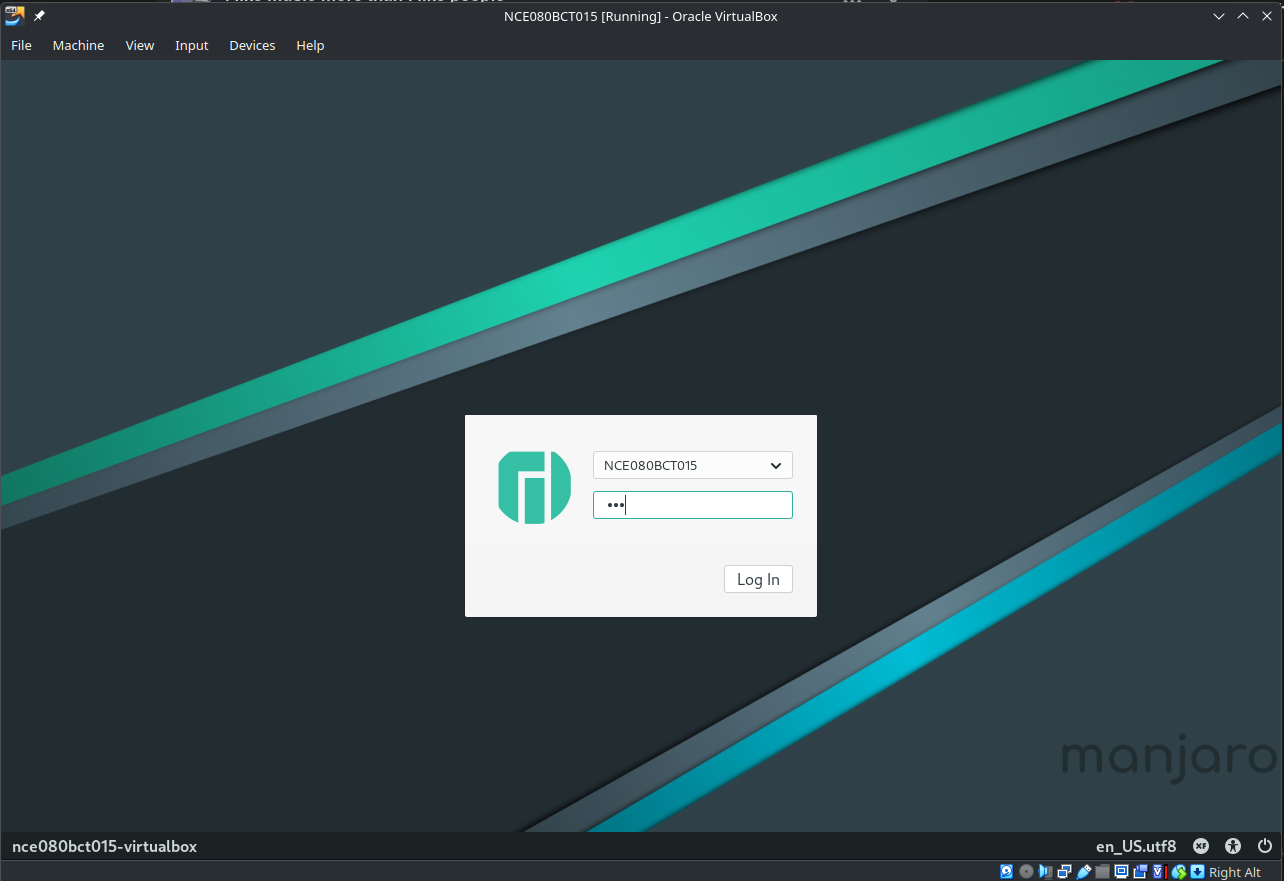
\includegraphics[width=0.7\linewidth]{post_install1.png}
    \caption{Post-Install boot}
    \label{fig19}
\end{figure}
\newpage
\begin{figure}[h]
    \centering
    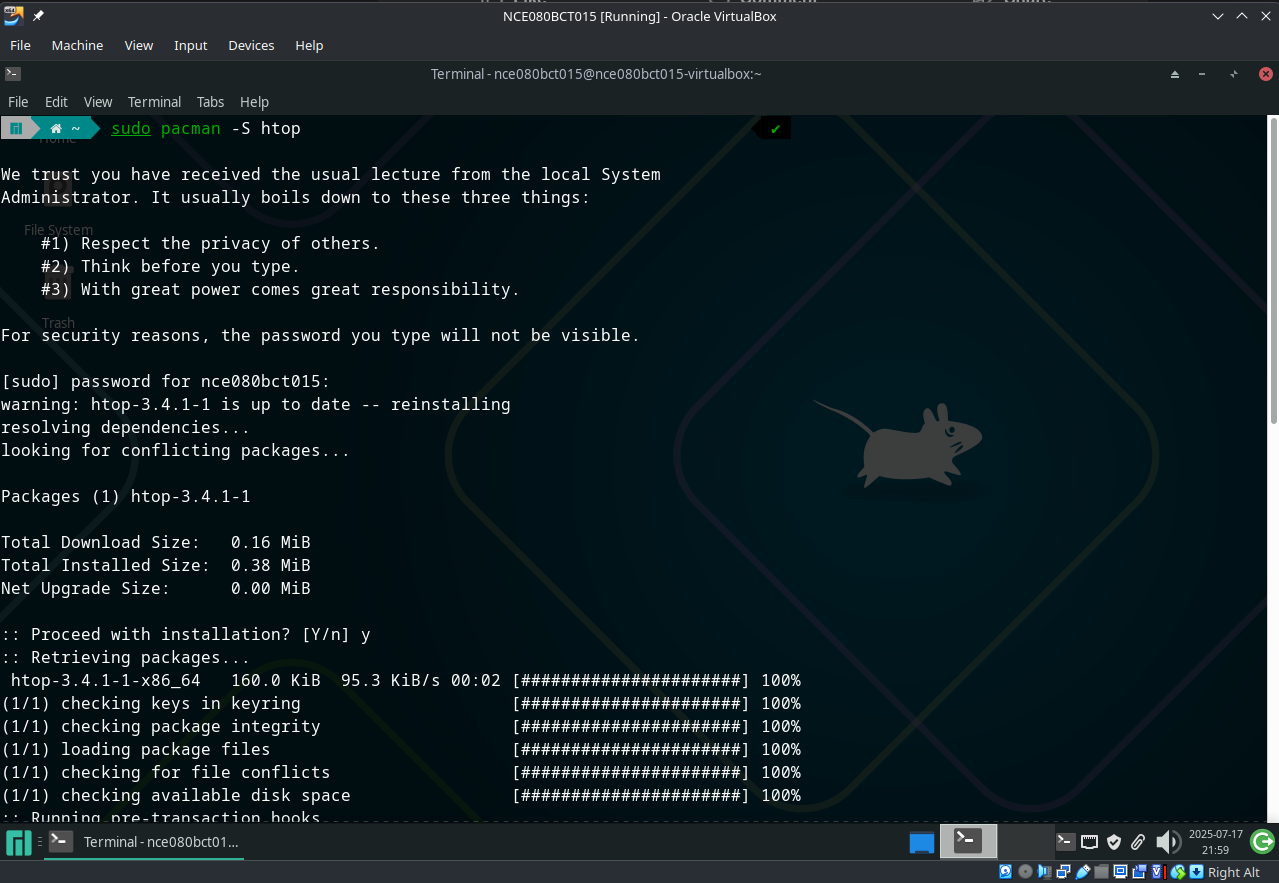
\includegraphics[width=0.6\linewidth]{post_install_config.png}
    \caption{Post-Install Config}
    \label{fig20}
\end{figure}
Installation of programs such as htop, neofetch was done using the terminal provided in Manjaro itself with the help of the Pacman package manager. 
\newpage
\begin{figure}[h]
    \centering
    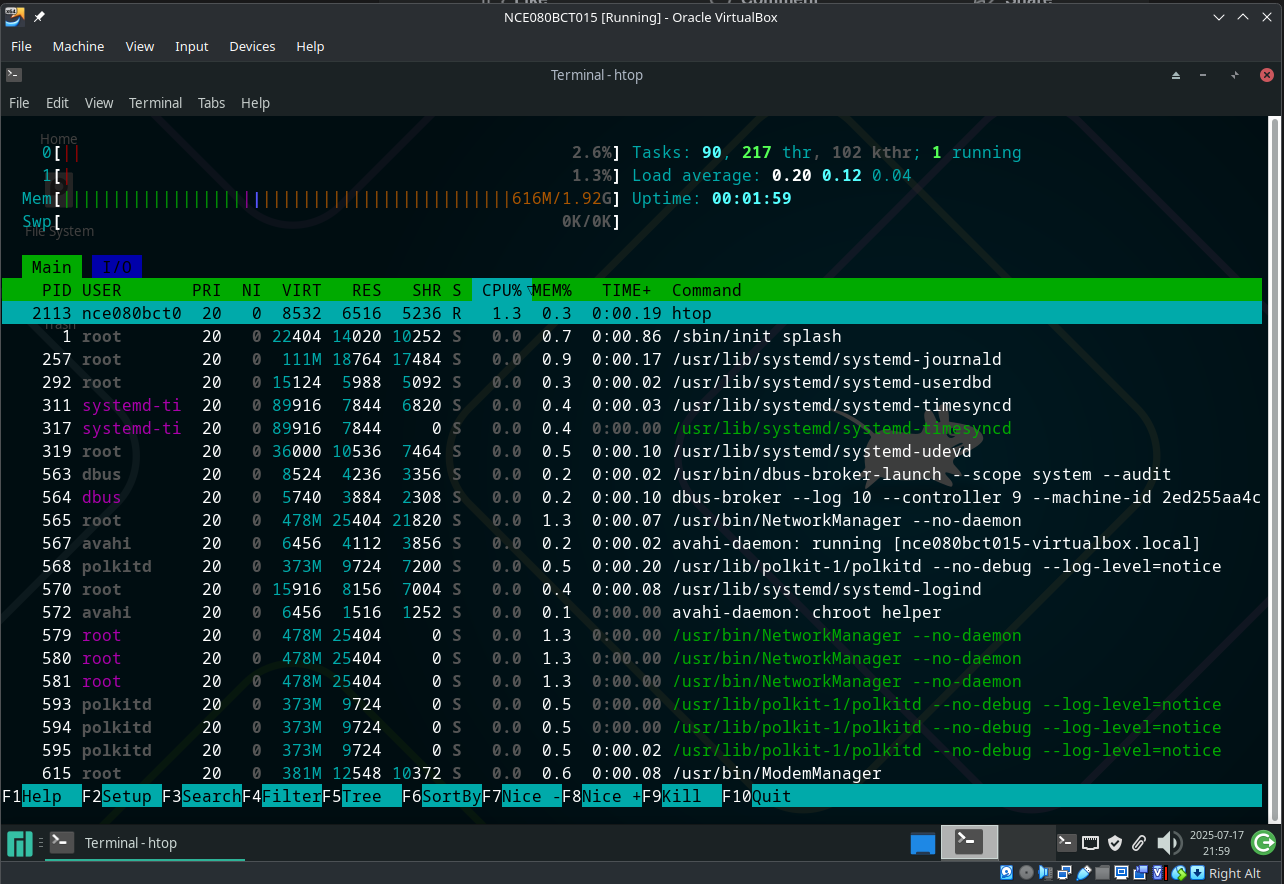
\includegraphics[width=0.6\linewidth]{post_install_config_2.png}
    \caption{Post-Install Config 2}
    \label{fig21}
\end{figure}
The use of htop to monitor the running processes showcased the resources we provided to the VirtualBox before installation which can be scaled through the settings menu.

\subsection{Pausing the VM}
Pausing the VM in Oracle's VirtalBox was relatively simple as it just required pressing the Host control key <R-Alt> and ll. 
\begin{figure}[h]
    \centering
    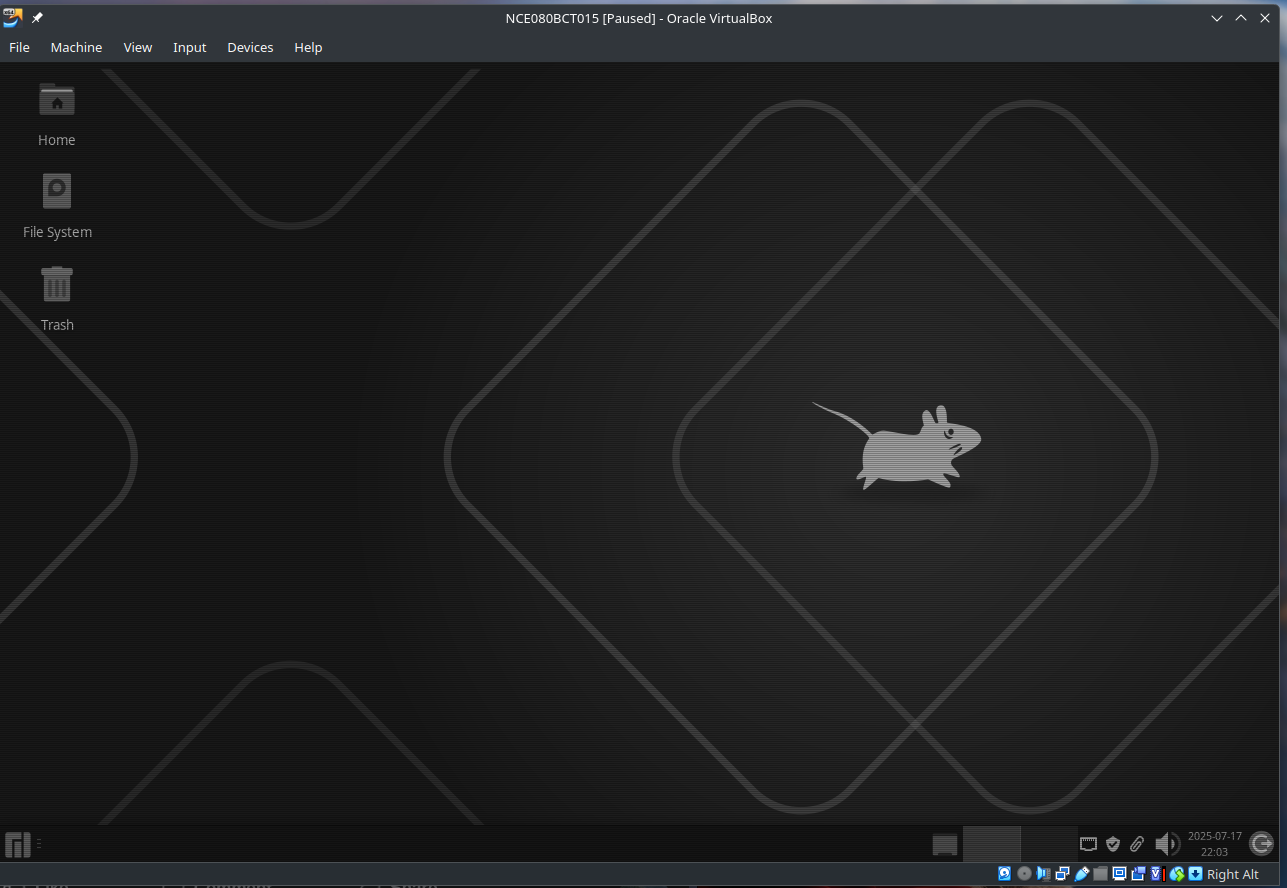
\includegraphics[width=0.7\linewidth]{pause.png}
    \caption{Paused VM}
    \label{fig22}
\end{figure}
\newpage
\subsection{Taking Snapshots}
Taking Snapshots in a VM is similar to reaching a checkpoint within a game where one can return to the checkpoint upon failure of the system. Snapshots function as a backup for users that want to install newer updates and run them on their system.
\begin{figure}[h]
    \centering
    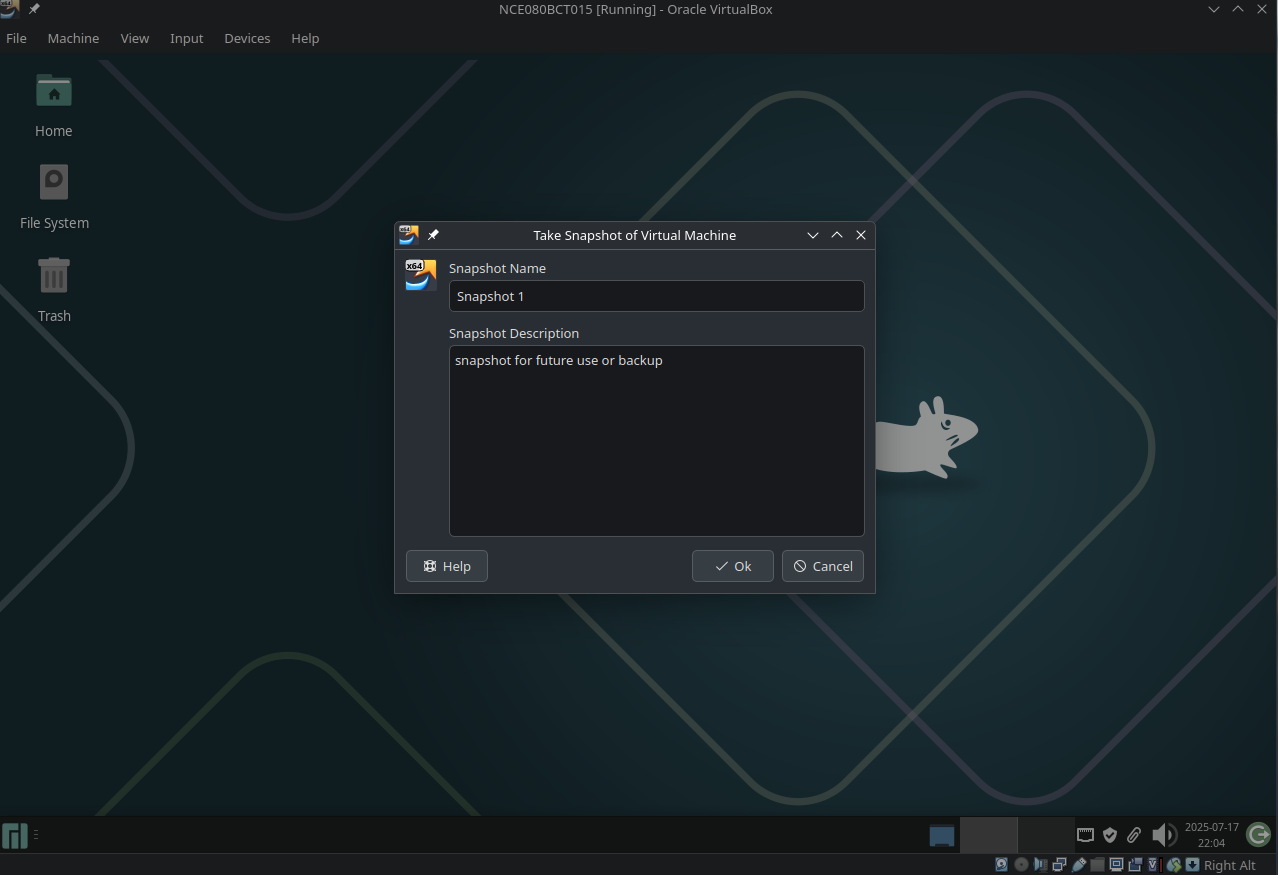
\includegraphics[width=0.7\linewidth]{snapshot.png}
    \caption{Taking a Snapshot}
    \label{fig23}
\end{figure}
\subsection{Exporting the VM}
Each virtualization software provides a way of exporting a VM, usually with the format Open Virtualization Formal (OVF)\footnotemark[1], which can be imported in any other virtualization software to create the same virtual machine.
Oracle VirtualBox provided an easy-to-use export feature.
\footnotetext[1]{OVA files are generally used and is the single-file archive that contains all the files of an OVF package}
\begin{figure}[h]
    \centering
    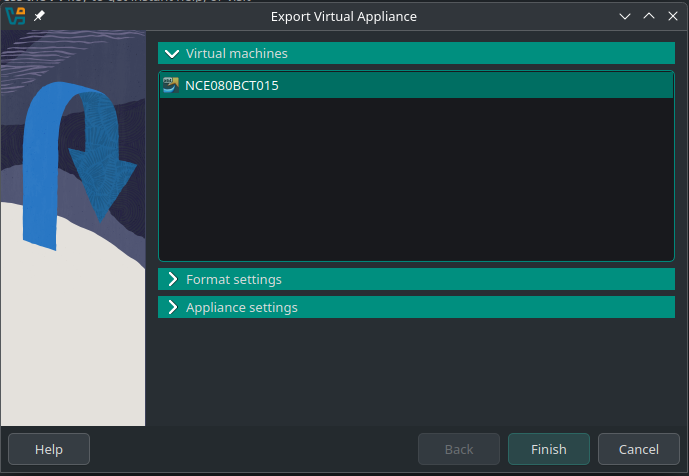
\includegraphics[width=0.5\linewidth]{export.png}
    \caption{Exporting the VM}
    \label{fig24}
\end{figure}
\newpage
\begin{figure}[h]
    \centering
    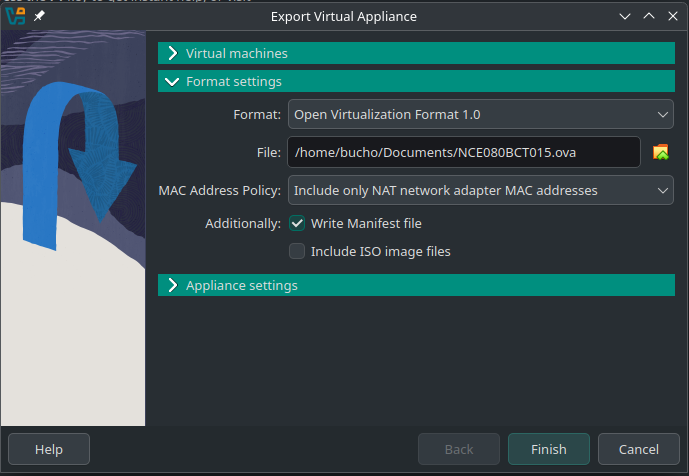
\includegraphics[width=0.5\linewidth]{export2.png}
    \caption{Export - Format Settings}
    \label{fig25}
\end{figure}
\begin{figure}[h]
    \centering
    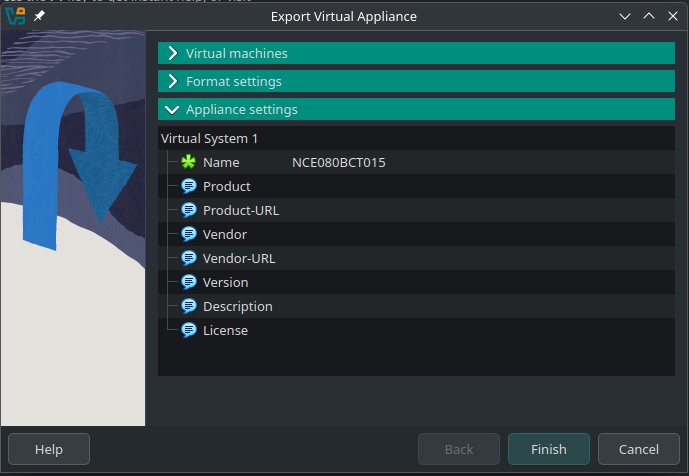
\includegraphics[width=0.5\linewidth]{export3.png}
    \caption{Export - Appliance Settings}
    \label{fig26}
\end{figure}
\newpage
\subsection{Importing a VM}
Importing any VM was similar to exporting. Any OVF file supported by VirtualBox could be imported and used as a Virtual Machine. 
Here, I demonstrated this feature by importing the same VM I exported.
\begin{figure}[h]
    \centering
    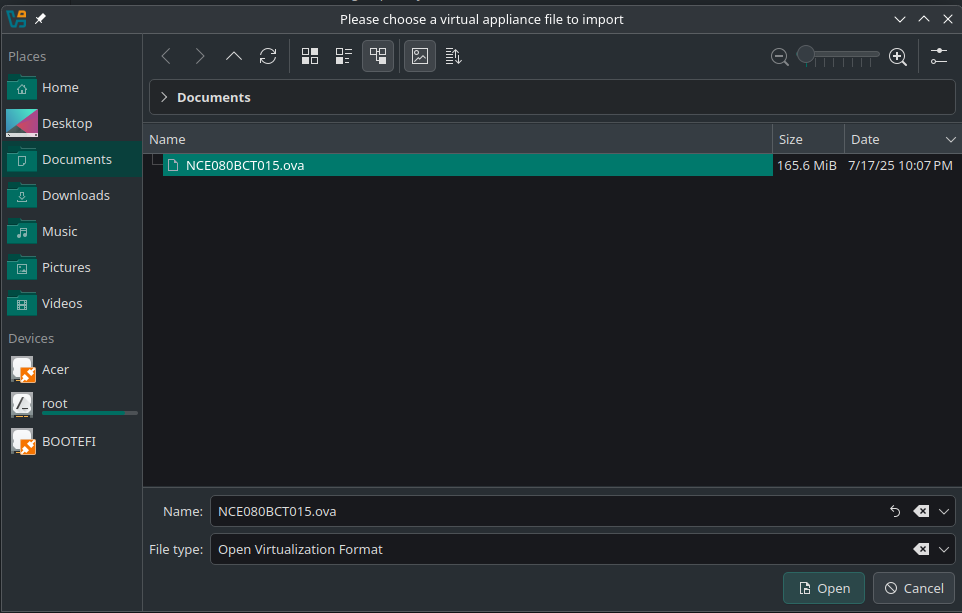
\includegraphics[width=0.5\linewidth]{import.png}
    \caption{Importing a VM}
    \label{fig27}
\end{figure}
\begin{figure}[h]
    \centering
    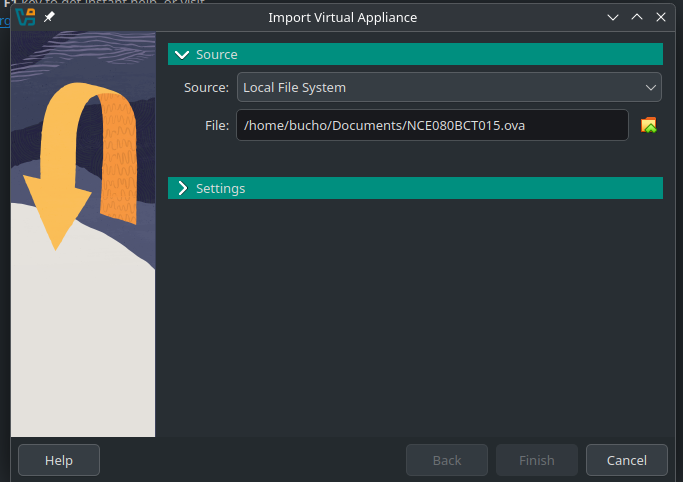
\includegraphics[width=0.5\linewidth]{import2.png}
    \caption{Import file}
    \label{fig27}
\end{figure}
\newpage
\subsection{Cloning the VM}
Cloning a VM means creating an exact copy(clone) of the machine. VirtualBox also provided an easy-to-use cloning feature. Here, I cloned my initial VM.
\begin{figure}[h]
    \centering
    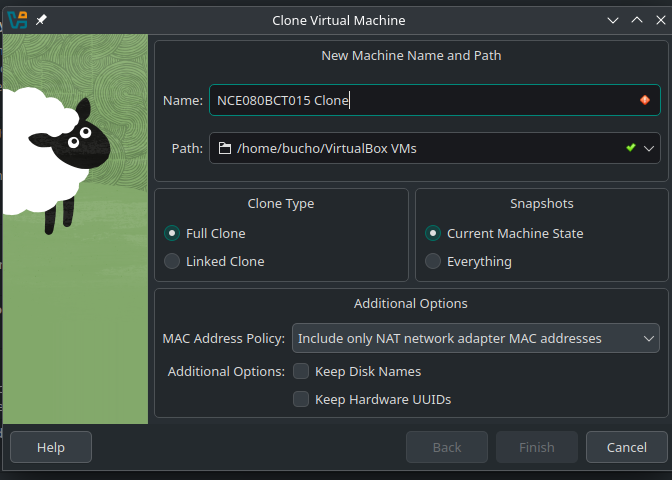
\includegraphics[width=0.5\linewidth]{clone.png}
    \caption{Cloning}
    \label{fig28}
\end{figure}
\section{Observation and Results}
Installing an OS on a VM and utilizing features such as cloning, importing, exporting and taking snapshots made me realize the ease and advantages of using a VM and virtualization instead of getting an extra machine.
\newline
Initially, if one knows how to install an OS on a bare metal, then knowing how to use a virtualization software to then create a VM lets him/her reap the benefits of virtualization.
I created a VM and installed Manjaro OS on it, and it was able to virtually create a system that replicated a physical system. 

\section{Advantages}
\section{Conclusion}


\end{document}
